\documentclass{article}
\usepackage[utf8]{inputenc}
\usepackage[spanish,es-nodecimaldot,es-tabla]{babel}
\usepackage{amsmath}
\usepackage{graphicx}
\usepackage[colorlinks=true, allcolors=blue]{hyperref}
\usepackage[makeroom]{cancel}
% hyperref para autoref, amsmath para split
\usepackage{subfig,placeins}
\usepackage{libertine}
\usepackage[libertine]{newtxmath}
\graphicspath{{./figs/}{./imgs/}}
\usepackage[font=small,labelfont=bf]{caption}
\usepackage{listings,figs/tuneatantito}
\newcommand\pder[2]{\ensuremath {\dfrac{\partial#1}{\partial#2}}} 
\newcommand{\ppder}[2]{ \ensuremath {\dfrac{\partial^2 #1}{\partial #2^2}}}
\newcommand{\ppcder}[3]{ \ensuremath {\dfrac{\partial^2 #1}{\partial #2\partial #3}}}

\title{Tarea 3}
\author{\href{https://git.io/salvador}{Pedraza-Espitia S.}}
\date{}

\begin{document}

\maketitle

\section{Corte meridional}
Realizar un programa que realice y grafique un corte meridional de U en donde se observe el
paso del huracán y guardar las gráficas de cuatro tiempos diferentes en formato jpg.


\lstinputlisting[language=Matlab]{./MatlabCodes/t3inciso1.m}
%\href{script1.txt}{Clic aquí para abrir script}
%\url{script1.m}
%%%%%
\begin{figure}[!ht]
\centering
  \hfill\subfloat[ii=24]{
  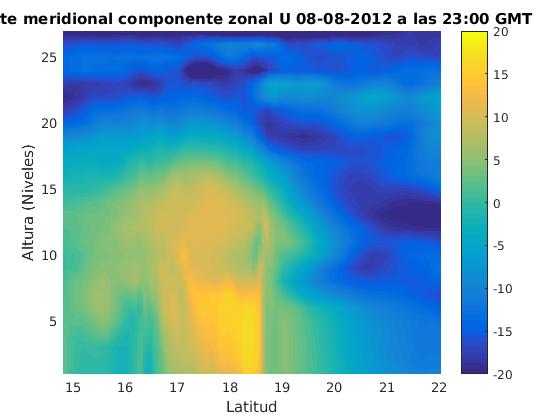
\includegraphics[width=0.35\textwidth]{t3fig24}
  }\hfill
  \subfloat[ii=29]{%\label{fig:}
  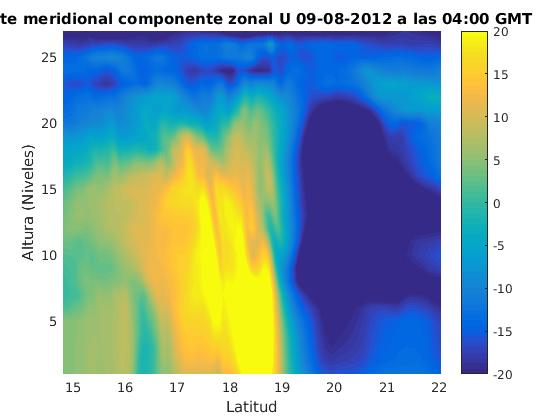
\includegraphics[width=0.35\textwidth]{t3fig29}
  }\hfill

  \hfill\subfloat[ii=34]{
  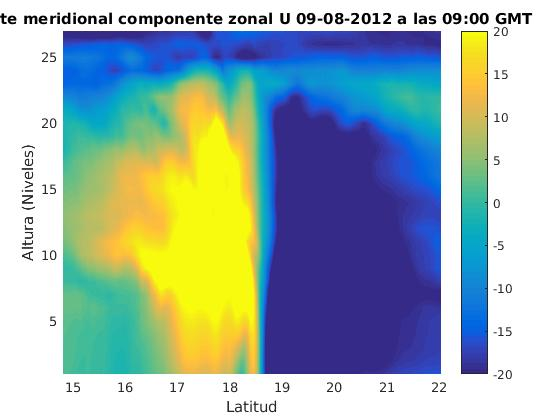
\includegraphics[width=0.35\textwidth]{t3fig34}
  }\hfill
  \subfloat[ii=39]{%\label{fig:}
  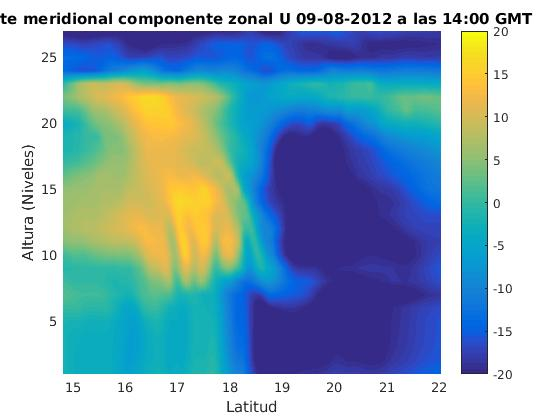
\includegraphics[width=0.35\textwidth]{t3fig39}
  }\hfill
  \caption{Evoluci\'on de la componente $U$ en un corte meridional (longitud fija $\approx$ -94$^o$)}%
\label{fig:uno}
\end{figure}
%%%%%

\section{Divergencia}
Hacer un programa que calcule la divergencia del viento a 10 metros, utilizando diferencias
finitas centradas, sin emplear funciones de matlab (DIV), y guardar las gráficas resultantes de
cuatro tiempos diferentes. Tomar en cuenta que la latitud y longitud que proporciona el
modelo están en grados y deberán convertirse a metros.

En la siguiente \autoref{sec:rotacional} se fusionan el ejercicio de obtener
divergencia y rotacional en un s\'olo script.
Las gr\'aficas que se piden se muestran en la \autoref{fig:dos}.
%%%%%
\begin{figure}[!ht]
\centering
  \hfill\subfloat[ii=24]{
  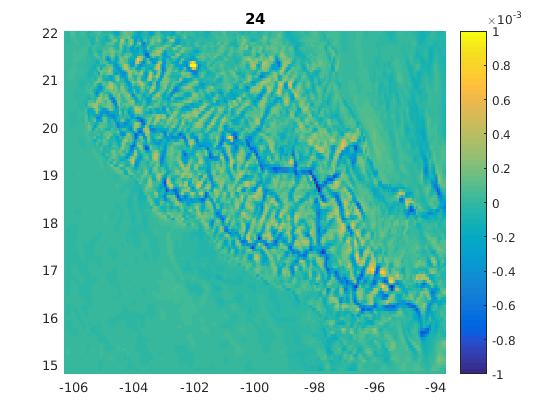
\includegraphics[width=0.35\textwidth]{t3div1}
  }\hfill
  \subfloat[ii=29]{%\label{fig:}
  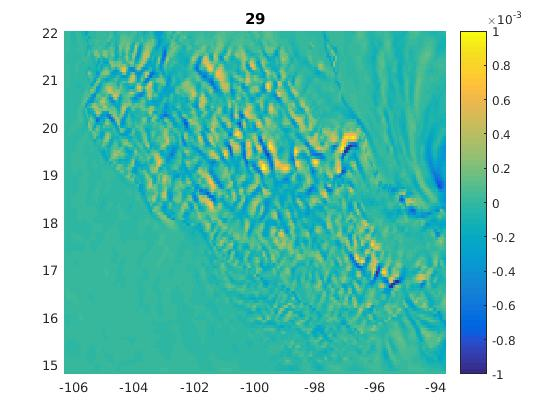
\includegraphics[width=0.35\textwidth]{t3div2}
  }\hfill

  \hfill\subfloat[ii=34]{
  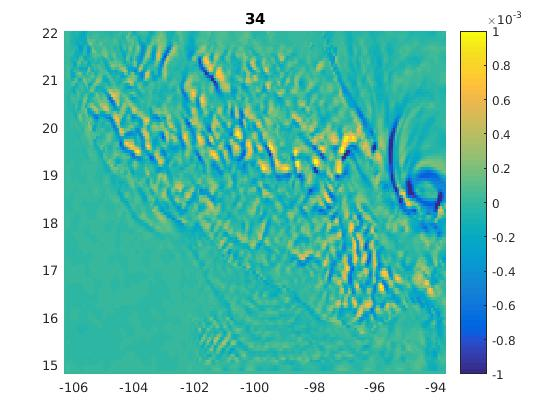
\includegraphics[width=0.35\textwidth]{t3div3}
  }\hfill
  \subfloat[ii=39]{%\label{fig:}
  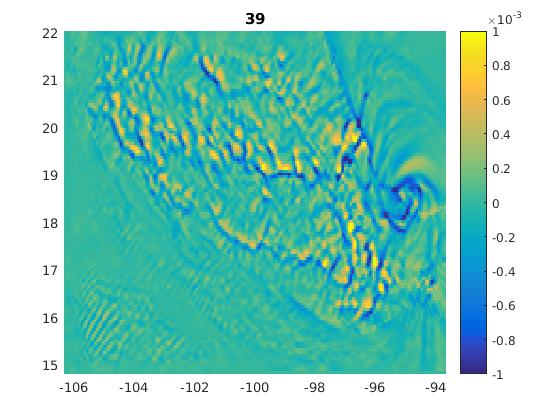
\includegraphics[width=0.35\textwidth]{t3div4}
  }\hfill
  \caption{Divergencia en 4 tiempos distintos, una divergencia positiva implica una fuente y una negativa indica hundimiento o sumidero.}%
\label{fig:dos}
\end{figure}
%%%%%

\section{Rotacional}\label{sec:rotacional}
Hacer un programa que calcule el rotacional del viento en el nivel 8, utilizando diferencias
finitas centradas, sin emplear funciones de matlab (CURL), y guardar las gráficas resultantes
de cuatro tiempos diferentes. Tomar en cuenta que la latitud y longitud que proporciona el
modelo están en grados y deberán convertirse a metros.
\lstinputlisting[language=Matlab]{./MatlabCodes/t3incisos2y3.m}
%%%%%
\begin{figure}[!ht]
\centering
  \hfill\subfloat[ii=24]{
  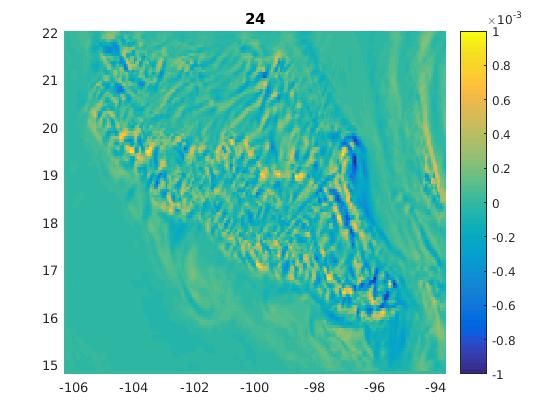
\includegraphics[width=0.35\textwidth]{t3rot1}
  }\hfill
  \subfloat[ii=29]{%\label{fig:}
  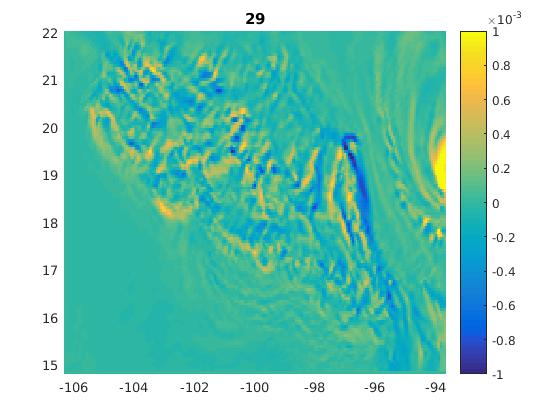
\includegraphics[width=0.35\textwidth]{t3rot2}
  }\hfill

  \hfill\subfloat[ii=34]{
  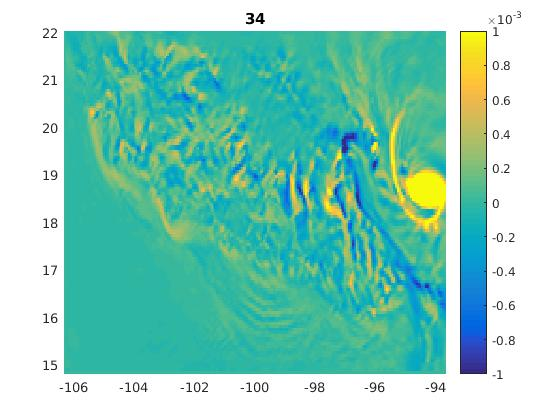
\includegraphics[width=0.35\textwidth]{t3rot3}
  }\hfill
  \subfloat[ii=39]{%\label{fig:}
  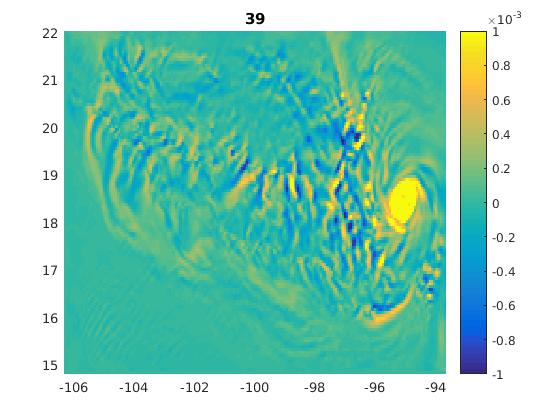
\includegraphics[width=0.35\textwidth]{t3rot4}
  }\hfill
  \caption{Rotacional en 4 tiempos distintos, se calcula sobre una superfice (nivel 8) y esto implica que s\'olo resulte una componente que es perpendicular a la superficie, el rotacional sigue la regla de la mano derecha y es proporcional a la velocidad angular.}%
\label{fig:tres}
\end{figure}
%%%%%
\FloatBarrier

\section{Resolver \texorpdfstring{$y' = cos(t)+sin(t)$}{y' = cos(t)+ ...} usando RK4}
Considera la ecuación diferencial $y' = cos(t) +sin(t)$ con $y(t=0) = 1$ y $h=0.1$.
Escribe un código
para calcular la solución con el método de Runge-Kutta de orden 4.
Recuerda que:
\begin{equation}
    \begin{split}
    k_1 = & h*f(t_i, y_i)\\
    k_2 = & h*f(t_i + h/2, y_i + k_1/2)\\
    k_3 = & h*f(t_i + h/2, y_i + k_2/2)\\
    k_4 = & h*f(t_i + h, y_i + k_3)
    \end{split}
    \nonumber
\end{equation}
\begin{equation}
    y_{i+1} = y_i + 1/6(k_1 + 2k_2 + 2k_3 + k_4)
    \label{eq:rec}
    \nonumber
\end{equation}

\lstinputlisting[language=Matlab]{./MatlabCodes/t3rk4_inciso4.m}
%%%%%
\begin{figure}[!hbt]
\centering
  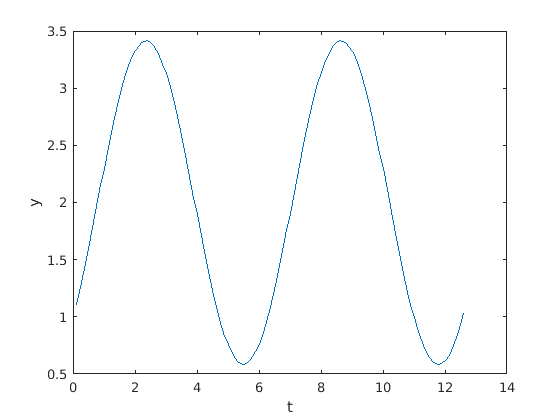
\includegraphics[width=0.6\textwidth]{t3inciso_4}
	\caption{Solución de $y'=\cos{t}+\sin{t}$.}%
	\label{fig:i4}
\end{figure}
%%%%%

\section{Resolver \texorpdfstring{$y'=y- 2*t^3 + 2$}{y'=y  2*t ...} con RK4}
Considera la ecuación diferencial $y' = y- 2*t^3 + 2$ con $y(t=0) = 0.5$.
Escribe un código para
calcular la solución con el método de Runge-Kutta de orden 4.

\lstinputlisting[language=Matlab]{./MatlabCodes/t3Rk4_inciso5.m}
%%%%%
\begin{figure}[!hbt]
\centering
  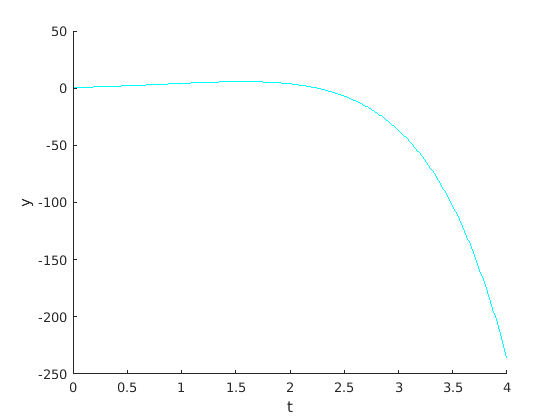
\includegraphics[width=0.6\textwidth]{t3inciso_5}
	\caption{Solución de $y'=y-2t^3+2$.}%
	\label{fig:i5}
\end{figure}
%%%%%

\section{Aguas soméras}

\begin{equation}
	\pder{u}{t} - fv = -g \pder{h}{x}
	\label{eq:uno}
\end{equation}

\begin{equation}
	\pder{v}{t} + fu = -g \pder{h}{y}
	\label{eq:dos}
\end{equation}

\begin{equation}
	\pder{h}{t} + H\left( \pder{u}{x} + \pder{v}{y} \right) = 0
	\label{eq:continuidad}%tres
\end{equation}

\begin{equation}
	\pder{[\eqref{eq:uno}]}{x} \Rightarrow
	\ppcder{u}{x}{t} - f\pder{v}{x} = -g \ppder{h}{x}
	\label{eq:cuatro}
\end{equation}

\begin{equation}
	\pder{[\eqref{eq:dos}]}{y} \Rightarrow
	\ppcder{v}{y}{t} + f\pder{v}{y} = -g \ppder{h}{y}
	\label{eq:cinco}
\end{equation}

\newcommand{\uymvx}{\left(\pder{u}{y}-\pder{v}{x}\right)}
\newcommand{\uxpvy}{\left(\pder{u}{x}+\pder{v}{y}\right)}
\newcommand{\hxphy}{\left(\ppder{h}{x}+\ppder{h}{y}\right)}

\begin{equation}
	[\eqref{eq:cuatro}+\eqref{eq:cinco}] \Rightarrow
	\pder{}{t}\uxpvy + f\uymvx = -g \hxphy
	\label{eq:seis}
\end{equation}

\begin{equation}
	\pder{[\eqref{eq:continuidad}]}{t} \Rightarrow
	\ppder{h}{t} + H\pder{}{t}\uxpvy = 0
	\label{eq:siete}
\end{equation}

\begin{equation}
    \begin{split}
	[\eqref{eq:siete}-H*\eqref{eq:seis}] \Rightarrow &
	\ppder{h}{t} + \cancel{H\pder{}{t}\uxpvy} -
	\cancel{H\pder{}{t}\uxpvy} \\
	& - Hf\uymvx = g \hxphy
    \end{split}
    \nonumber
\end{equation}
\begin{equation}
    \Rightarrow \ppder{h}{t} - Hf\uymvx
	 -gH \hxphy = 0
    \label{eq:ocho}
\end{equation}

\begin{equation}
	\pder{[\eqref{eq:uno}]}{y} \Rightarrow
	\ppcder{u}{y}{t} - f\pder{v}{y} = -g \ppcder{h}{y}{x}
	\label{eq:nueve}
\end{equation}

\begin{equation}
	\pder{[\eqref{eq:dos}]}{x} \Rightarrow
	\ppcder{v}{x}{t} + f\pder{u}{x} = -g \ppcder{h}{x}{y}
	\label{eq:diez}
\end{equation}

\begin{equation}
	[\eqref{eq:nueve}+\eqref{eq:diez}] \Rightarrow
	\pder{}{t} \uymvx = f \uxpvy
	\label{eq:once}
\end{equation}

\begin{equation}
	[\eqref{eq:continuidad}] \Rightarrow
	\uxpvy = -\frac1H \pder{h}{t}
	\label{eq:tres.uno}
\end{equation}

\begin{equation}
	[\eqref{eq:tres.uno} \text{ y } \eqref{eq:once}] \Rightarrow
	\pder{}{t} \uymvx = -f\frac1H \pder{h}{t}
	\label{eq:doce}
\end{equation}

\begin{equation}
	\pder{[\eqref{eq:ocho}]}{t} \Rightarrow
	\pder{}{t}\ppder{h}{t} - Hf\pder{}{t}\uymvx - gH \pder{}{t}\hxphy = 0
	\label{eq:trece}
\end{equation}

\begin{equation}
	[\eqref{eq:once} \text{ y } \eqref{eq:trece}] \Rightarrow
	\pder{}{t}\ppder{h}{t}
	- Hf^2\uxpvy - gH \pder{}{t}\hxphy = 0
	\label{eq:catorce}
\end{equation}

\begin{equation}
	[\eqref{eq:tres.uno} \text{ y } \eqref{eq:catorce}] \Rightarrow
	\pder{}{t}\ppder{h}{t}
	- Hf^2 \left(-\frac1H \pder{h}{t}\right) - gH \pder{}{t}\hxphy = 0
	\label{eq:quince}
\end{equation}

\begin{equation}
	\pder{}{t}\ppder{h}{t}
	+ f^2 \left(\pder{h}{t}\right) - gH \pder{}{t}\hxphy = 0
\end{equation}
\begin{equation}
	\pder{}{t}\left[\ppder{}{t}
	+ f^2 - gH\left(\ppder{}{x}+\ppder{}{y}\right)\right]h = 0
\end{equation}

\end{document}